\section{Visualization}
%

\noindent\textbf{MOT20.} OmniTrack is a MOT framework specifically designed for panoramic FoV, facilitating target localization and association across distorted and panoramic FoV images. Unlike pinhole cameras, where objects tend to be denser, panoramic images typically feature more sparsely distributed targets. To intuitively demonstrate OmniTrack's performance in dense pedestrian scenarios, we visualize its tracking results on sequence 07 of the MOT20 test set~\cite{dendorfer2020mot20}, as shown in Fig.~\ref{fig:MOT20}. The results indicate that OmniTrack successfully tracks most targets; however, it struggles with particularly small or heavily occluded objects, such as the one next to ID 20. The primary challenge stems from the limited training data in MOT20~\cite{dendorfer2020mot20}, which contains only $4$ sequences, posing a significant challenge for $OmniTrack_{Det}$. In future work, we aim to enhance tracking performance in dense target scenarios.

\noindent\textbf{QuadTrack \& JRDB.} We visualize the final tracking results on the JRDB~\cite{martin2021jrdb} and QuadTrack datasets, as shown in Fig.~\ref{fig:vis_img_jrdb} and Fig.~\ref{fig:vis_img_quadtrack}. 
In these images, red arrows highlight instances where trajectories were lost and not correctly tracked, while yellow arrows indicate identity confusion, leading to ID switches. In Fig.~\ref{fig:vis_img_jrdb}, for the JRDB dataset~\cite{martin2021jrdb}, we observe that OmniTrack accurately tracks objects, even in scenes with a large number of people, without any ID switches or trajectory losses. 
In contrast, ByteTrack~\cite{zhang2022bytetrack} and SORT~\cite{bewley2016simple} both exhibit trajectory losses, while OC-SORT~\cite{cao2023observation} experiences multiple ID switches. 
In Figure~\ref{fig:vis_img_quadtrack}, for the QuadTrack dataset, the tracking of cyclists in the foreground remains intact, while OC-SORT, ByteTrack, and SORT all suffer from trajectory loss at frame $247$. These examples demonstrate OmniTrack's superior recall ability, further validating the effectiveness of our feedback mechanism and the FlexiTrack Instance in accurately maintaining targets in panoramic-FoV scenarios.

\begin{figure*}[!t]
  \centering
  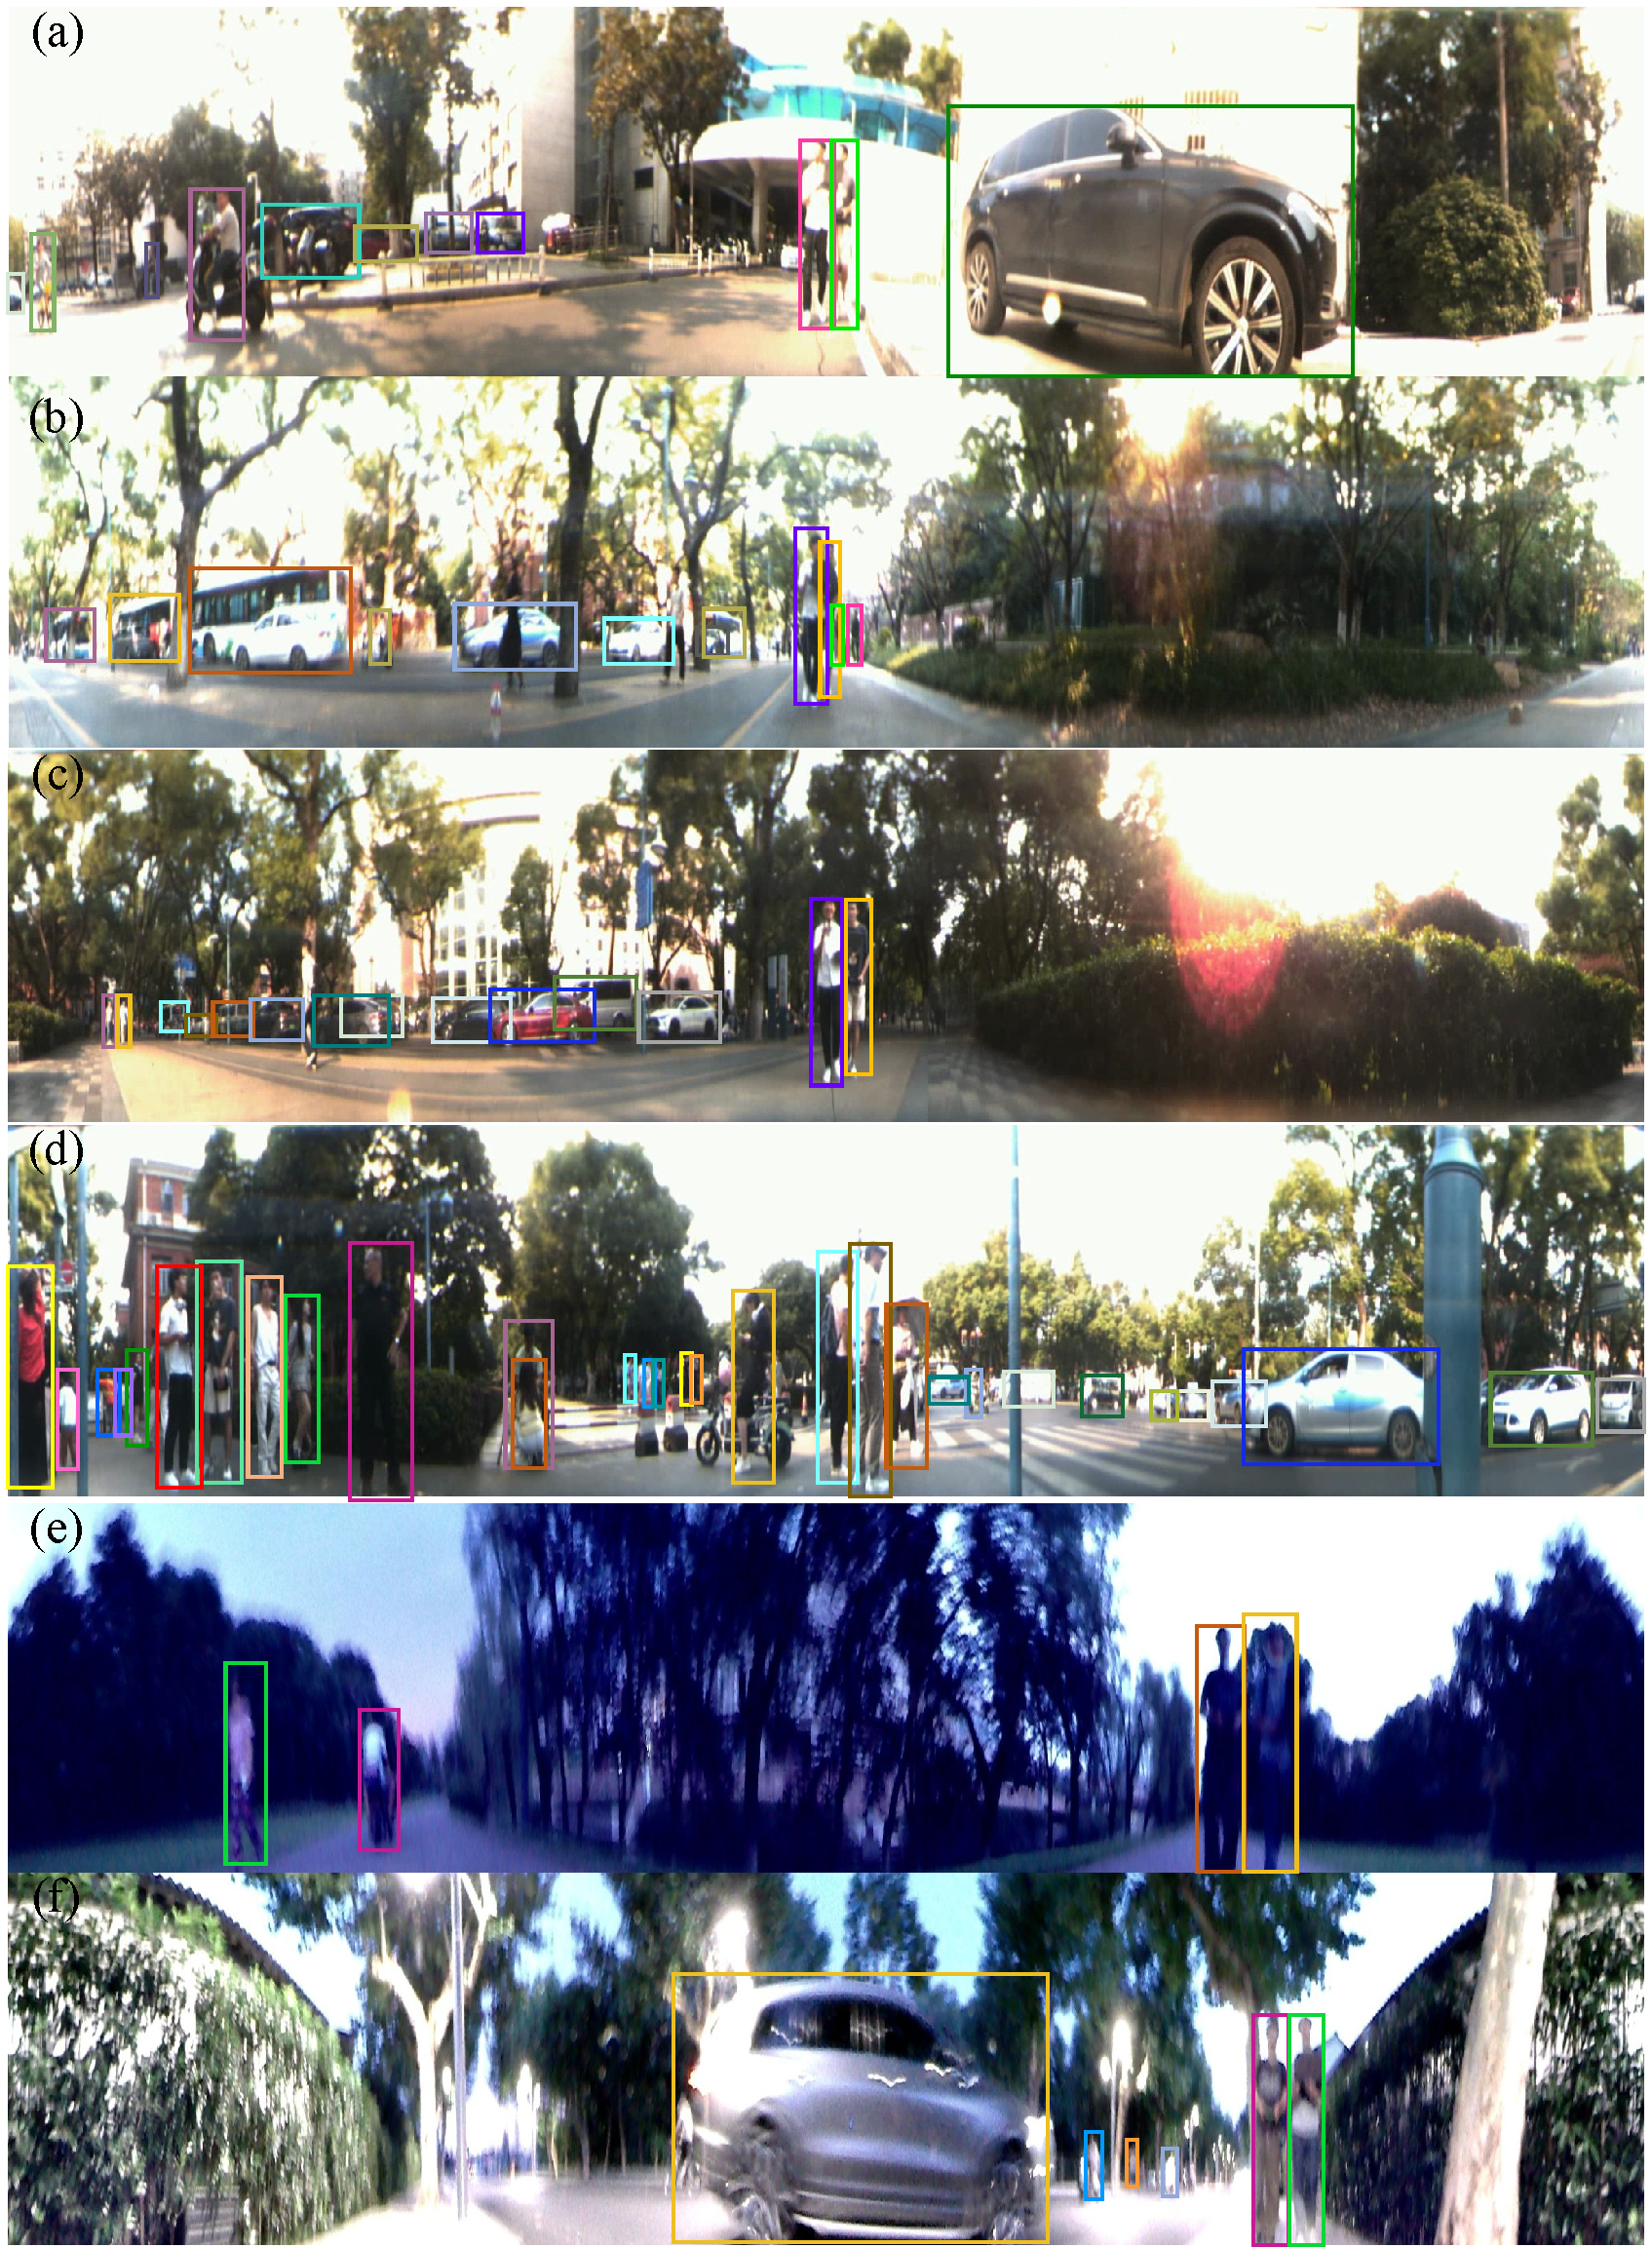
\includegraphics[width=0.80\textwidth]{imgs/vis_img_v2.pdf}
  %\vskip -2ex
  \caption{Examples of the established QuadTrack dataset. The QuadTrack dataset features a variety of scenes, including different campuses, streets, and low-light environments, with machine-generated labels for each scenario. These labeled scenes demonstrate the diversity and complexity of the dataset, offering insights into the challenges of multi-object tracking across different real-world contexts.}
  \label{fig:vis_anno}
  %\vskip -2ex
\end{figure*}

\begin{figure*}[!t]
  \centering
  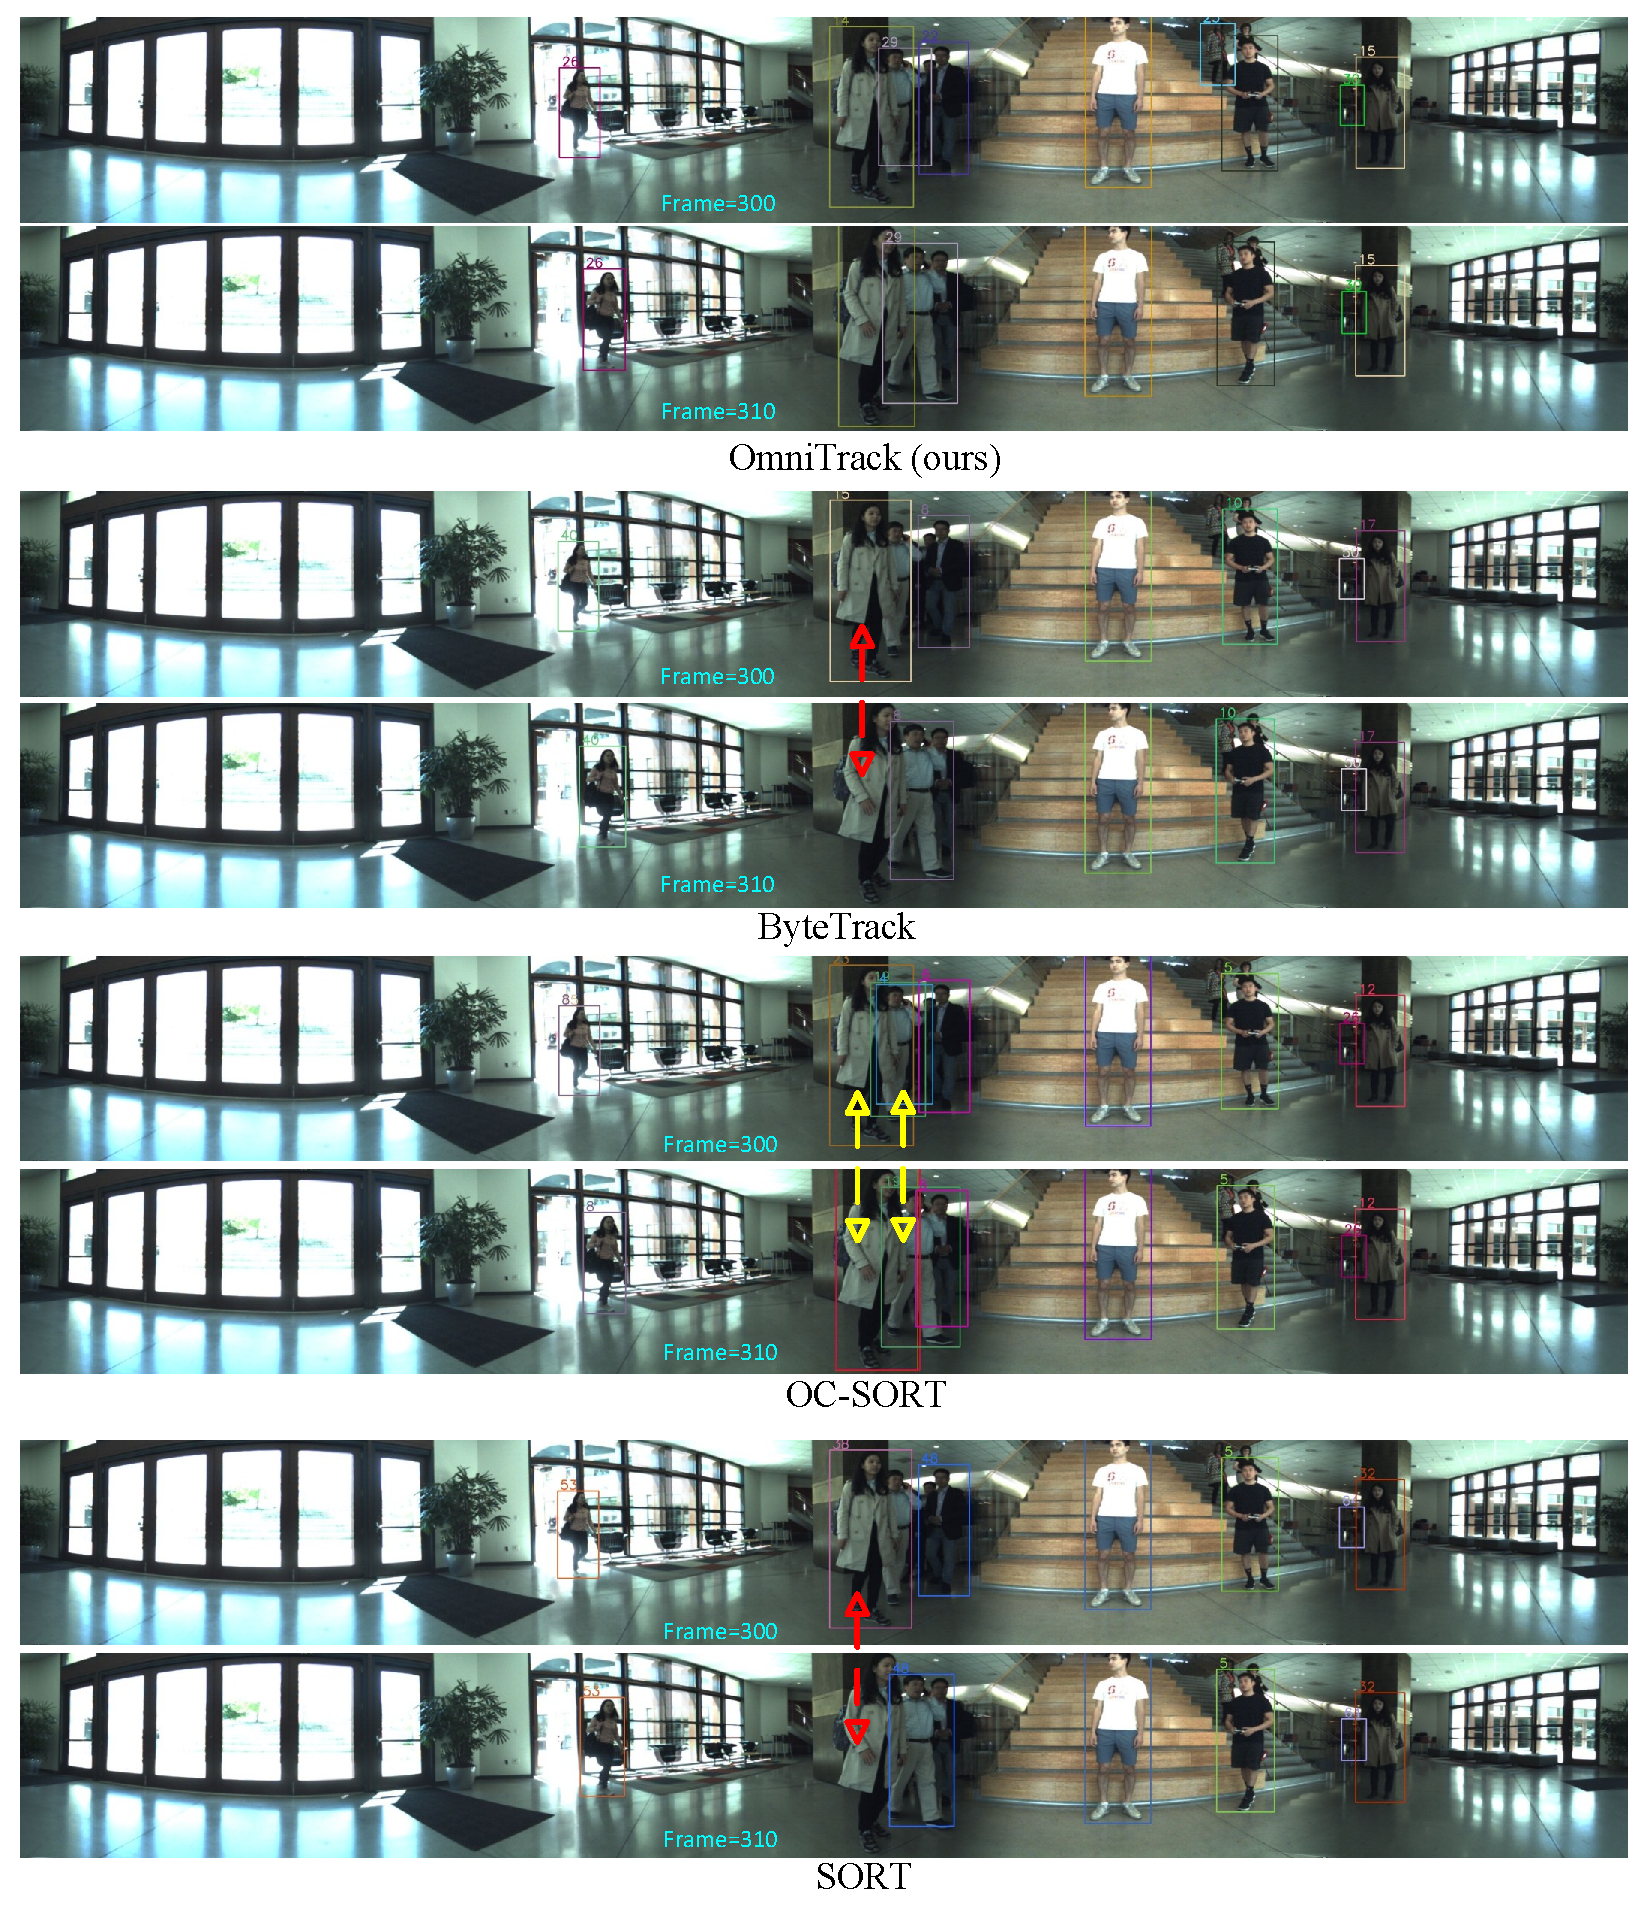
\includegraphics[width=0.98\textwidth]{imgs/jrdb_tracking_vis_2.pdf}
  %\vskip -2ex
  \caption{Visualization on the public JRDB dataset~\cite{martin2021jrdb}. The visualization compares the performance of OmniTrack, SOTA~\cite{bewley2016simple}, ByteTrack~\cite{zhang2022bytetrack}, and OC-SORT~\cite{cao2023observation} methods on the JRDB validation set. The \textcolor{red}{red} arrows in the figures indicate instances where the trajectories were not correctly tracked, leading to tracking losses, while \textcolor{yellow}{yellow} arrows highlight cases of track ID confusion, indicating ID switches.}
  \label{fig:vis_img_jrdb}
  %\vskip -2ex
\end{figure*}


\begin{figure*}[!t]
  \centering
  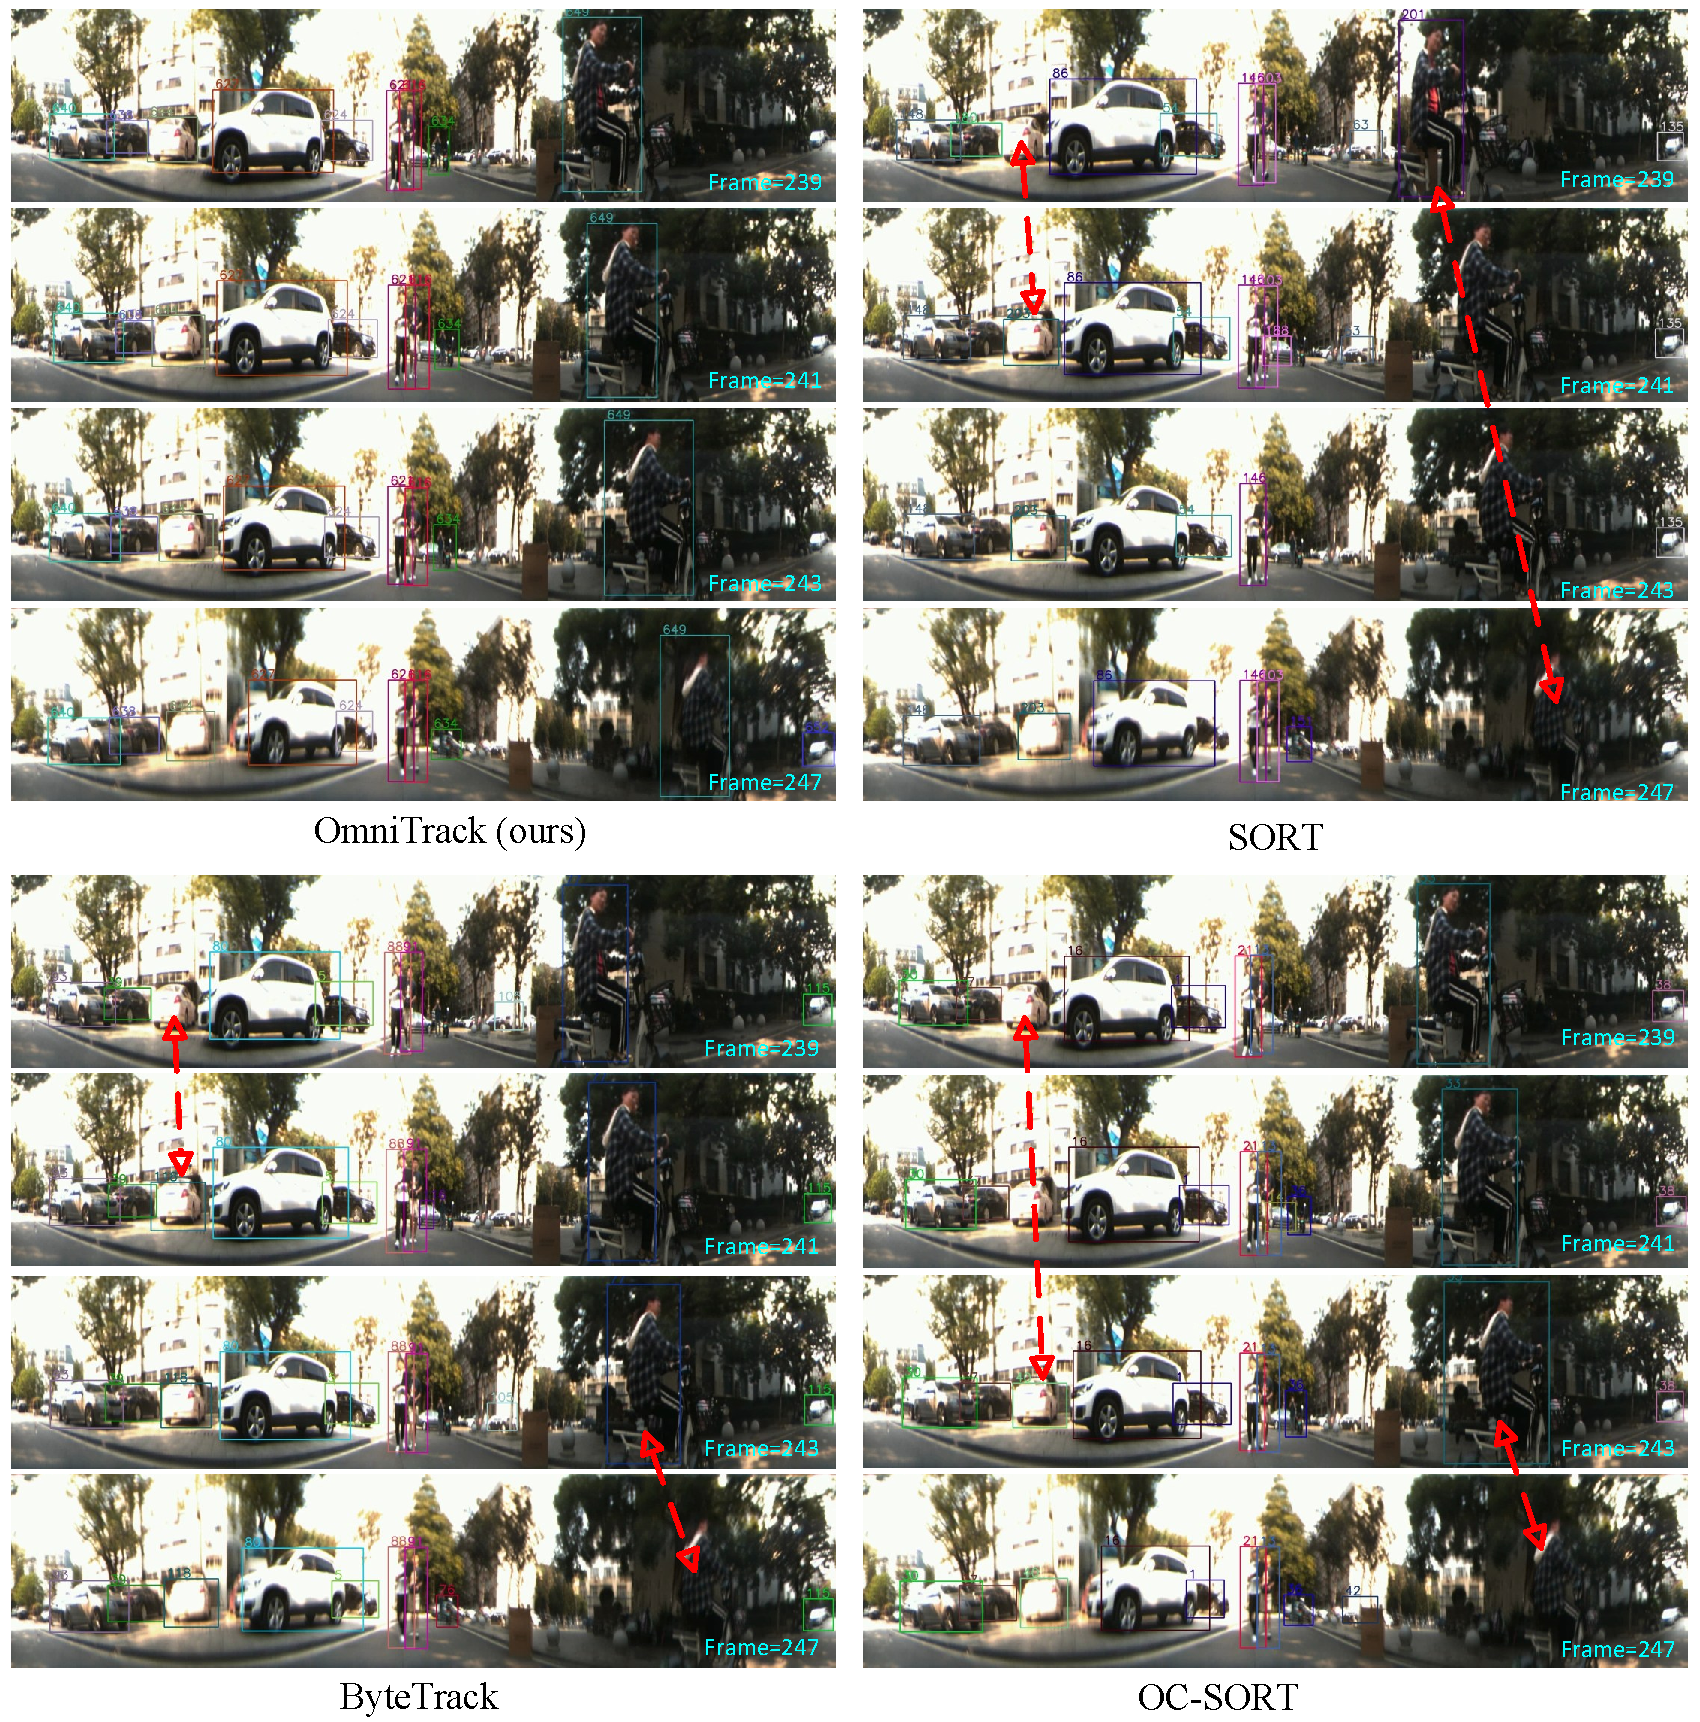
\includegraphics[width=1\textwidth]{imgs/tracking_vis_v3_2.pdf}
  %\vskip -2ex
  \caption{Visualization comparison on the established QuadTrack dataset. The visualization compares the performance of OmniTrack, SOTA~\cite{bewley2016simple}, ByteTrack~\cite{zhang2022bytetrack}, and OC-SORT~\cite{cao2023observation} methods on the QuadTrack test set. The \textcolor{red}{red} arrows in the figures indicate instances where the trajectories were not correctly tracked, leading to tracking losses.}
  \label{fig:vis_img_quadtrack}
  %\vskip -2ex
\end{figure*}

%
